\section{Exercises}
\label{s:exercises}

\subsection{Rate estimate of stellar-mass binary black hole mergers}
\label{exer:1}

Estimate the total rate (number of events per time) of 
stellar-mass binary black hole mergers throughout the universe 
by multiplying LIGO's O1 local rate 
estimate $R_0 \sim 10$~-~$200~{\rm Gpc}^{-3}\,{\rm yr}^{-1}$ by 
the comoving volume out to some large redshift, e.g., $z= 10$.
(For this calculation you can ignore any dependence of the 
rate density with redshift.)
You should find a merger rate of $\sim\!1$~per minute to a few 
per hour.
{\em Hint}: You will need to do numerically evaluate the
following integral for proper distance today as a function 
of source redshift:
%
\be
d_0(z) = \frac{c}{H_0}\int_0^z\frac{\D z'}{E(z')}\,,
\qquad
E(z)\equiv \sqrt{\Omega_{\rm m}(1+z)^3 + \Omega_\Lambda}\,,
\ee
%
with 
%
\be
\Omega_{\rm m}=0.31\,,
\qquad
\Omega_\Lambda=0.69\,,
\qquad
H_0 = 68~{\rm km}\,{\rm s}^{-1}\, {\rm Mpc}^{-1}\,.
\ee
Doing that integral, you should find what's shown in
Figure~\ref{f:d0vsz}, which you can then evaluate at
$z=10$ to convert $R_0$ (number of events per 
comoving volume per time) to total rate (number of 
events per time) for sources out to redshift $z=10$.
%
\begin{figure}[htbp!]
\begin{center}
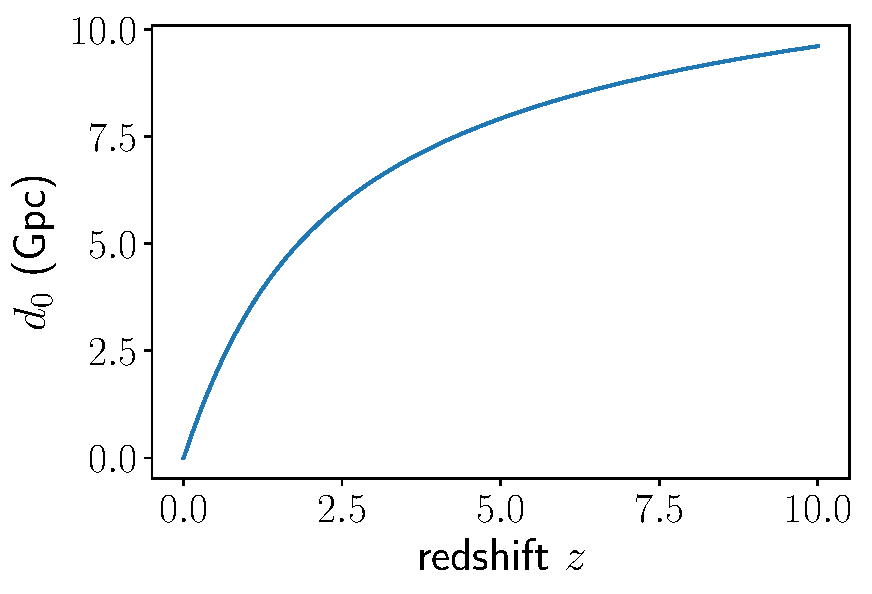
\includegraphics[width=0.5\textwidth]{Figures/d0vsz}
\caption{}
\label{f:d0vsz}
\end{center}
\end{figure}
%

\subsection{Relating $S_h(f)$ and $\Omega_{\rm gw}(f)$}
\label{exer:2}

Derive the relationship 
\be
S_h(f) = \frac{3 H_0^2}{2\pi^2}\frac{\Omega_{\rm gw}(f)}{f^3}
\ee
between the strain power spectral density $S_h(f)$ and the 
dimensionless fractional energy density spectrum $\Omega_{\rm gw}(f)$.
({\em Hint}: You will need to use the various definitions of these
quantities and also 
\be
\rho_{\rm gw} =\frac{c^2}{32\pi G}\langle \dot h_{ab}(t,\vec x)\dot h^{ab}(t,\vec x)\rangle\,,
\ee
which expresses the energy-density in gravitational-waves to 
the metric perturbations $h_{ab}(t,\vec x)$.)

\subsection{Cosmology and the ``Phinney formula" for astrophysical backgrounds}
\label{exer:3}

(a) Using the Friedmann equation
%
\be
\left(\frac{\dot a}{a}\right)^2
=H_0^2\left(\frac{\Omega_{\rm m}}{a^{3}} + \Omega_\Lambda\right)
\ee
%
for a spatially-flat FRW spacetime with matter and 
cosmological constant, and the relationship 
%
\be
1+z = \frac{1}{a(t)}\,,
\qquad a(t_0)\equiv 1\quad(t_0\equiv {\rm today})\,,
\ee
%
between redshift $z$ and scale factor $a(t)$,
derive 
%
\be
\frac{\D t}{\D z} =-\frac{1}{(1+z)H_0 E(z)}\,,
\qquad
E(z) = \sqrt{\Omega_{\rm m}(1+z)^3 + \Omega_\Lambda}\,.
\ee
%
(b) Using this result for $\D t/\D z$, show that 
%
\be
\Omega_{\rm gw}(f)= \frac{f}{\rho_{\rm c}H_0}
\int_0^\infty \D z\>R(z)\,\frac{1}{(1+z)E(z)}
\left(\frac{\D E_{\rm gw}}{\D f_{\rm s}}\right)\bigg|_{f_{\rm s}=f(1+z)}
\ee
%
in terms of the rate density $R(z)$ as measured in 
the source frame 
(number of events per comoving volume per time interval
in the source frame).
({\em Hint}: The expression for $\D t/\D z$ from part
(a) will allow 
you to go from the ``Phinney formula" for
$\Omega_{\rm gw}(f)$ written in terms of the number 
density $n(z)$,
%
\be
\Omega_{\rm gw}(f)= \frac{1}{\rho_c}\int_0^\infty \D z\>
n(z)\,\frac{1}{1+z}\left(f_{\rm s}\,
\frac{\D E_{\rm gw}}{\D f_{\rm s}}\right)\bigg|_{f_{\rm s}=f(1+z)}\,,
\ee
%
to one in terms of the rate density 
$R(z)$, where $n(z)\,\D z=R(z)\,|\D t|_{t=t(z)}$.
Note: Both of the above expressions for $\Omega_{\rm gw}(f)$
assume that there is only one type of source, described by 
some set of average source parameters.  
If there is more than one type of source, one must sum
the contributions of each source to $\Omega_{\rm gw}(f)$.)

\subsection{Optimal filtering for the cross-correlation statistic}
\label{exer:4}

Verify the form 
%
\be
\tilde Q(f)\propto \frac{\Gamma_{12}(f)H(f)}
{P_1(f)P_2(f)}\,,
\ee
of the optimal filter function in the weak-signal limit,
where $H(f)$ is the assumed spectral shape of the 
gravitational-wave background,
$\Gamma_{12}(f)$ is the overlap function, and $P_1(f)$, $P_2(f)$ 
are the power spectral densities of the outputs of the 
two detectors (which are approximately equal to 
$P_{n_1}(f)$, $P_{n_2}(f)$, respectively).
Recall that the optimal filter $\tilde Q(f)$ maximizes
the signal-to-noise ratio of the cross-correlation 
statistic.
({\em Hint}: Introduce an inner product on the space of
functions of frequency $A(f)$, $B(f)$:
%
\be
(A,B)\equiv\int df A(f) B^*(f) P_1(f) P_2(f)\,.
\ee
%
This inner product
has all of the properties of the familiar dot product
of vectors in 3-dimensional space.
The signal-to-noise ratio of the cross-correlation
statistic can be written in terms of this inner product.)

\subsection{Maximum-likelihood estimators for single and multiple
parameters}
\label{exer:5}

(a) Show that the maximum-likelihood estimator $\hat a$ of 
the single parameter $a$ in the likelihood function
\be
p(d|a, \sigma) \propto
\exp\left[-\frac{1}{2}\sum_{i=1}^N \frac{(d_i-a)^2}{\sigma_i^2}\right]
\ee
%
is given by the noise-weighted average
%
\be
\hat a={\sum_i \frac{d_i}{\sigma_i^2}}\bigg/{\sum_j \frac{1}{\sigma_j^2}}\,.
\ee
%
(b) Extend the previous calculation to the likelihood
\be
p(d|A, C) \propto
\exp\left[-\frac{1}{2}(d-MA)^\dagger C^{-1} (d-MA)\right]\,,
\ee
%
where $A\equiv A_\alpha$ is a vector of parameters,
$C\equiv C_{ij}$ is the noise covariance matrix, and 
$M\equiv M_{i\alpha}$ is the response matrix mapping 
$A_\alpha$ to data samples, $MA\equiv \sum_\alpha M_{i\alpha}A_\alpha$.
For this more general case you should find:
%
\be
\hat A = F^{-1} X\,,
\ee
%
where
%
\be
F \equiv M^\dagger C^{-1} M\,,\qquad
X \equiv M^\dagger C^{-1} d\,.
\ee
%
In general, the matrix $F$ (called the {\em Fisher} matrix)
is not invertible, so some sort of regularization is needed
to do the matrix inversion.

\subsection{Timing-residual response for a 1-arm, 1-way detector}
\label{exer:6}

Derive the timing residual reponse function
%
\be
R^A(f,\hat k) = 
\frac{1}{2}u^a u^b e^A_{ab}(\hat k)
\frac{1}{i2\pi f}
\frac{1}{1-\hat k\cdot \hat u}
\left[1-e^{-\frac{i2\pi fL}{c}(1-\hat k\cdot\hat u)}\right]
\ee
%
for a single-link (i.e., a one-arm, one-way detector like 
that for pulsar timing).
Here $\hat u$ is the direction of propagation of the
electromagnetic pulse, and $\hat k$ is the direction of
propagation of the GW (the direction to the GW source is
$\hat n\equiv -\hat k$, and the direction to the pulsar is
$\hat p\equiv -\hat u$).
The origin of coordinates is taken to be at the position 
of the detector.

\subsection{Overlap function for colocated electric dipole antennae}
\label{exer:7}

Show that the overlap function for a pair of (short)
colocated electric dipole antennae pointing in directions 
$\hat u_1$ and $\hat u_2$ (Figure~\ref{f:dipole-orf})
is given by 
%
\be
\Gamma_{12} 
%\equiv \langle r_1 r_2\rangle
\propto
\hat u_1\cdot\hat u_2 
\equiv\cos\zeta
\ee
% 
for the case of an unpolarized, isotropic electromagnetic field.
({\em Hint}: ``short" means that the phase of the electric 
field can be taken to be constant over of the lengths of 
the dipole antennae, 
so that the reponse of antenna $I=1,2$ to the field is
given by $r_I(t)=\hat u_I\cdot\vec E(t, \vec x_0)$, where
$\vec x_0$ is the common location of the two antenna.)
 
\subsection{Maximum-likelihood estimators for the standard 
cross-correlation statistic}
\label{exer:8}

Verify that 
%
\be
\hat C_{11}\equiv \frac{1}{N}\sum_{i=1}^N d_{1i}^2\,,
\qquad
\hat C_{22}\equiv \frac{1}{N}\sum_{i=1}^N d_{2i}^2\,,
\qquad
\hat C_{12}\equiv \frac{1}{N}\sum_{i=1}^N d_{1i} d_{2i}
\ee
%
are maximum-likelihood estimators of 
%
\be
S_1\equiv S_{n_1}+S_h\,,
\quad
S_2\equiv S_{n_2}+S_h\,,
\quad
S_h\,,
\ee
for the case of $N$ samples of a white GWB in uncorrelated
white detector noise, for a pair of colocated and coaligned 
detectors.
Recall that the likelihood function is
%
\be
p(d|S_{n_1}, S_{n_2}, S_h) =\frac{1}{\sqrt{{\rm det}(2\pi C)}}
\exp\left[-\frac{1}{2}d^T C^{-1} d\right]\,,
\ee
%
where
\be
C
= \left[
\begin{array}{cc}
(S_{n_1} +S_h)\,\unit_{N\times N} & S_h\,\unit_{N\times N}
\\
S_h\,\unit_{N\times N} & (S_{n_2} +S_h)\,\unit_{N\times N}
\\
\end{array}
\right]
\label{e:C_marginalized}
\ee
%
and 
%
\be
d^T C^{-1} d
\equiv \sum_{I,J=1}^2\sum_{i,j=1}^N
d_{Ii} \left(C^{-1}\right)_{Ii,Jj} d_{Jj}\,.
\label{e:argexp}
\ee

\subsection{Derivation of the maximum-likelihood ratio detection statistic}
\label{exer:9}

Verify that twice the log of the maximum-likelihood
ratio for the standard stochastic likelihood function
goes like the square of the (power) signal-to-noise ratio,
\be
2\ln \Lambda_{\rm ML}(d) \simeq
\frac{\hat C_{12}^2}{\hat C_{11}\hat C_{22}/N}\,,
\ee
in the weak-signal approximation.
({\em Hint:} For simplicity, do the calculation in the context 
of $N$ samples of a white GWB in uncorrelated 
white detector noise, for a pair of colocated and coaligned
detectors, using the results of Exercise~\ref{exer:8}.)

\subsection{Standard cross-corr likelihood marginalizing over 
stochastic signal prior}
\label{exer:10}

Derive the standard form of the likelihood function
for stochastic background searches 
\be
p(d|S_{n_1}, S_{n_2}, S_h)
=\frac{1}{\sqrt{{\rm det}(2\pi C)}}
\exp\left[-\frac{1}{2} \sum_{I,J=1}^2 d_I \left(C^{-1}\right)_{IJ} d_J\right]\,,
\ee
%
where
%
\be
C\equiv \left[
\begin{array}{cc}
S_{n_1}+S_h & S_h\\
S_h & S_{n_2} + S_h\\
\end{array}
\right]\,,
\ee
by marginalizing 
\be
p_n(d- h|S_{n_1},S_{n_2}) =
\frac{1}{2\pi\sqrt{S_{n_1}S_{n_2}}}
\exp\left[-\frac{1}{2}\left\{
\frac{(d_1- h)^2}{S_{n_1}} + \frac{(d_2- h)^2}{S_{n_2}}
\right\}\right]
\ee
over the signal samples $h$ for the {\em stochastic} signal prior 
\be
p(h|S_h) = \frac{1}{\sqrt{2\pi S_h}}\exp\left[
-\frac{1}{2}\frac{h^2}{S_h}\right]\,.
\ee
%
In other words, show that
%
\be
p(d|S_{n_1}, S_{n_2}, S_h) 
=\int_{-\infty}^\infty \D h\>
p_n(d-h|S_{n_1}, S_{n_2}) p(h|S_h)\,.
\ee
%
({\em Hint}: You'll have to complete the square in the argument
of the exponential in the marginalization integral.)

